
\documentclass[a4paper,14pt]{extarticle}

\usepackage[utf8]{inputenc}
\usepackage[T1]{fontenc}
\usepackage[english,russian]{babel}
\usepackage[oglav,spisok,boldsect,eqwhole,figwhole,hyperref,hyperprint,remarks,greekit]{./style/fn2dipstyle}
\graphicspath{{./style/}{./figures/}}

\usepackage{setspace}
\setstretch{1.5}
\usepackage[left=3cm,right=1cm, top=2cm,bottom=2cm]{geometry}
\usepackage{pdfpages}
\pagestyle{plain}
\usepackage{mathtools}

% Центрированные таблицы фиксированной ширины %
\usepackage{tabularx} % also loads 'array' package
\newcolumntype{C}{>{\centering\arraybackslash}X} % centered version of 'X' columns

\usepackage{relsize}
\newcommand{\smallalpha}{\mathsmaller{(} \alpha \mathsmaller{)}}
\newcommand{\smallbeta}{\mathsmaller{(} \beta \mathsmaller{)}}
\newcommand{\avg}[1]{\left\langle #1 \right\rangle}
\usepackage[titles]{tocloft}

\usepackage{multirow}
\usepackage{supertabular}
\usepackage{multicol}
\usepackage{amsmath}
\usepackage{afterpage}
\usepackage{amsmath}
% Параметры титульного листа
%\title{Решение уравнения Рейнольдса\\ в рамках теории газовой смазки \\ методом конечных элементов}
%\author{В.\,Г.~Пиневич}
%\supervisor{А.\,В.~Селиванов}
%\group{ФН2-81Б}
%\date{2024}

% Переопределение команды \vec, чтобы векторы печатались полужирным курсивом
\renewcommand{\vec}[1]{\text{\mathversion{bold}${#1}$}}%{\bi{#1}}
\newcommand\thh[1]{\text{\mathversion{bold}${#1}$}}
%Переопределение команды нумерации перечней: точки заменяются на скобки
\renewcommand{\labelenumi}{\theenumi)}
\begin{document}
	
	
\section-{Реферат}	

Расчетно-пояснительная записка 60 с., 41 рис., 1 табл., 22 источника, 2
прил.

МЕТОД КОНЕЧНЫХ ЭЛЕМЕНТОВ, УРАВНЕНИЕ РЕЙНОЛЬДСА,
ГАЗОВАЯ СМАЗКА, ПАЛЬЧИКОВОЕ УПЛОТНЕНИЕ.

Продемонстрирована возможность построения многодисциплинарной ма-
тематической модели пальчикового уплотнения на основе объединения моде-
ли Рейнольдса для течения в тонких пленках между валом и невращающимся
надроторным кольцом и балочной модели расчета НДС гибкого подвеса сег-
ментного кольца. Модель может быть использована для экспресс-анализа ра-
боты пальчикового уплотнения на этапе предварительного проектирования.

Хорошее качественное и количественное согласование численных результатов, полученных с помощью разработанной программы решения уравнения Рейнольдса методом конечных элементов, с известными аналитическими решениями для уравнений Лапласа и Пуассона подтверждает возможность использования программы при определении распределений давления в
тонких пленках жидкости.

Деформирование пальчиков под действием газовых нагрузок приводит
к образованию раскрывающегося зазора, что негативно влияет на несущую
способность подъемных площадок и снижает эффективность уплотнения.
Для предотвращения этого эффекта целесообразно располагать пальчики с
предварительным наклоном к поверхности ротора для образования сходящегося по окружности зазора.

\newpage

\tableofcontents



\newpage

\section{Введение}
Задачи расчёта подшипников газодинамического типа с зазорами разнообразной формы до сих пор остаются весьма актуальными. По сути, они сводятся к изучению газового смазочного слоя в тонком зазоре произвольной формы. Решением таких задач занимается гидродинамическая теория смазки. Этот раздел механики жидкости и газа начал развиваться в конце XIX века вслед за потребностями техники. Начало теоретическому исследованию течений в тонких зазорах положили работы Н. П. Петрова и британского учёного Осборна Рейнольдса, уточнённые и доведённые до возможности практического применения А. Зоммерфельдом, А. Мичелем. Дальнейшие исследования позволили распространить результаты созданной Рейнольдсом теории на газодинамические подшипники. Были даже предприняты успешные попытки получения общего вида уравнения Рейнольдса для смазочного слоя без привязки к конкретной системе координат. Данная работа посвящена получению пригодной к использованию в практических задачах формы уравнения Рейнольдса и решению его методом конечных элементов.


\subsection{Постановка задачи}
Задача данной работы --- вывести, а затем показать методику решение дифференциального уравнения Рейнольдса методом конечных элементов.
\begin{equation}
	\label{reinolts-task}
\frac{\partial}{\partial x} \left(h^3 \frac{\partial p}{\partial x} \right) + \frac{\partial}{\partial z} \left(h^3 \frac{\partial p}{\partial z} \right) = 6 \mu U \frac{\partial h}{\partial x} \text{, }
\end{equation}
где $h = h(x)$ --- толщина слоя, $p = p(x, z)$ --- давление, $\mu$ --- коэффициент вязкости. Граничные условия: $U$ --- скорость в направлении $x$ на одной из пластин, $p_{\text{в}}$ --- повышенное давление, $p_{\text{н}}$ --- пониженное давление. 

Размеры области зададим 5 мм по ширине и 5 мм по длине. Будем использовать коэффициент вязкости воды $\mu = 8.90 \cdot 10^{-4} \text{ Па} \cdot \text{с}$.
\newline Давление возьмем $p_{\text{н}} = 100 \text{ кПа}, p_{\text{в}} = 150 \text{ кПа}$. Скорость будет меняться в зависимости от специфики расчетов. Схематичное изображение области задачи и граничных условий изображено на рис.~\ref{obl_resh}.

\begin{figure}[!htbp]
	\center{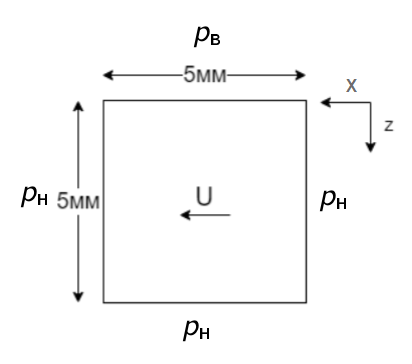
\includegraphics[width=\textwidth, height=0.5\textwidth]{taskGU.png}}
	\caption{Схема области решения и граничных условий уравнения Рейнольдса}
	\label{obl_resh}
\end{figure}

\subsection{Получение уравнения Рейнольдса}

Уравнение Рейнольдса является одним из основных уравнений в области механики жидкостей и газов. Оно было названо в честь физика Осгуда Рейнольдса, который впервые сформулировал его в середине XIX века.
Уравнение Рейнольдса имеет широкое применение в различных областях науки и техники, таких как гидродинамика, аэродинамика, теплообмен. Это уравнение является основой для предсказания и анализа различных явлений, связанных с течением жидкостей и газов.
Гидродинамические уравнения несжимаемой жидкости с
внутренним трением могут быть представлены в очень простой
форме, если пренебречь силами, пропорциональными массам,
равно как и силами инерции.

Обозначая через $x$, $y$, $z$ прямоугольные координаты точки, через $p$ -- гидродинамическое давление в этой точке,

Силы трения $p_{xy}, p_{xz}, p_{yx}, p_{yz}, p_{zx}, p_{zy}$, перпендикулярные к оси силы, обозначенной первой буквой индекса и параллельные оси силы, обозначенной второй буквой индекса.

Обозначим проекции скорости на осях $x, y, z \text{ соответственно}$ $u, \nu, \omega$.

Введем $\mu$ как коэффициент внутреннего трения жидкости.ы
 Тогда можно записать три системы уравнений:
\begin{enumerate}
	\item Система, определяющая гидродинамическое давление в
	точке $x, y, z$:
	\begin{equation}
		\label{eqfi}
		\begin{cases}
			\frac{\partial p}{\partial x} = \mu \left( \frac{\partial^2 u}{\partial x^2} + \frac{\partial^2 u}{\partial y^2} + \frac{\partial^2 u}{\partial z^2} \right), \\
				\frac{\partial p}{\partial y} = \mu \left( \frac{\partial^2 \nu}{\partial x^2} + \frac{\partial^2 \nu}{\partial y^2} + \frac{\partial^2 \nu}{\partial z^2} \right), \\
					\frac{\partial p}{\partial z} = \mu \left( \frac{\partial^2 \omega}{\partial x^2} + \frac{\partial^2 \omega}{\partial y^2} + \frac{\partial^2 \omega}{\partial z^2} \right).
		\end{cases}
	\end{equation}
\item Система, определяющая силы трения в той же точке:
\begin{equation}
	\label{eqsi}
	\begin{cases}
		p_{yz} = p_{zy} = \mu \left(\frac{\partial \omega}{\partial y} + \frac{\partial \nu}{\partial z} \right), \\
			p_{zx} = p_{xz} = \mu \left( \frac{\partial \omega}{\partial x} +  \frac{\partial u}{\partial z} \right), \\
				p_{xy} = p_{yx} = \mu \left(  \frac{\partial u}{\partial y} + \frac{\partial \nu}{\partial x} \right).
	\end{cases}
\end{equation}
\item Условие несжимаемости жидкости, выраженное уравнением: 
\begin{equation}
	\label{eqthi}
	\frac{\partial u}{\partial x} + \frac{\partial \nu}{\partial y} + \frac{\partial \omega}{\partial z} = 0.
	\end{equation}

\end{enumerate}

Примем, что скорость $\nu = 0$, поскольку она мала по сравнению со скоростями $u = 0$, $\omega = 0$.

Изменения скоростей $u$ и $\omega$ со при заданном значении $y$ для всех изменений $ x $ и $z$ могут рассматриваться как чрезмерно малые, поэтому примем
\[
\frac{\partial^2 u}{\partial x^2} = 0, 
\frac{\partial^2 u}{\partial z^2} = 0, 
\frac{\partial^2 \omega}{\partial x^2} = 0, 
\frac{\partial^2 \omega}{\partial z^2} = 0. 
\]

Ограничиваясь приближенным решением, которое можно
получить при указанных выше предположениях, уравнения \eqref{eqfi}, \eqref{eqsi} и \eqref{eqthi} могут быть приведены к следующей форме.
\begin{equation}
	\label{secondinitialeq}
	\begin{cases}
		\frac{\partial p }{\partial x} = \mu \frac{\partial^2 u}{\partial y^2}, \\
		\frac{\partial p }{\partial y} = 0, \\
		\frac{\partial p }{\partial z} = \mu \frac{\partial^2 \omega}{\partial y^2}.
	\end{cases}
\end{equation}
\begin{equation}
	\label{secinitialeq}
	\begin{cases}
		p_{yz} = p_{xy} = \mu \frac{\partial \omega}{\partial y}, \\
		p_{zx} = p_{xz} = 0, \\
		p_{xy} = p_{yx} = \mu \frac{\partial u}{\partial y}.
	\end{cases}
\end{equation}
\begin{equation*}
	\frac{\partial u}{\partial x} + \frac{\partial \nu}{\partial y} + \frac{\partial \omega}{\partial z} = 0.
\end{equation*}

Для определения давления необходимо интегрировать выражения \eqref{secondinitialeq}, \eqref{secinitialeq}. Для этого определим граничные условия.

\noindent Для $y = 0$ имеем
\[
\begin{cases}
u = U_0, \\
 \nu = 0, \\
  \omega = 0.
\end{cases}
\]

\noindent Для $y = h$ имеем
\[
\begin{cases}
u = U_1, \\ 
\nu = U_1 - U_1 \frac{\partial  h}{\partial h}, \\ \omega = 0.
\end{cases}
\]

Поскольку $p$ не зависит от $y$, то интегрирование уравнений \eqref{secondinitialeq} приводит к уравнениям
\begin{equation}
	\label{1-inte-inti}
	\begin{cases}
		u = \frac{1}{2 \mu} \frac{\partial p}{\partial x} \left( y - h \right) y + U_0 \frac{h - y}{h} + U_1 \frac{y}{h},\\
		\omega = \frac{1}{2 \mu} \frac{\partial p}{\partial z} (y - h) y.
	\end{cases}
\end{equation} 
Первые производные вторых членов этих уравнений, перенесенные в соответствующие уравнения группы \eqref{secinitialeq}, приводят
к уравнениям
\begin{equation}
	\label{sec-init-eq}
	\begin{cases}
		p_{yz} = p_{zy} = \frac{1}{2} \frac{\partial p}{\partial z} \left( 2y - h \right), \\
		p_{xy} = p_{yz} = \frac{1}{2} \frac{\partial p}{\partial x} \left( 2y - h \right) + \mu \frac{U_1 - U_0}{h}.
	\end{cases}
\end{equation}

Если давление $p$ считать независимым от координаты $z$, то четыре последних
уравнения сокращаются до двух: первое из системы~\eqref{1-inte-inti} и
второе из системы~\eqref{sec-init-eq}.

Взяв производные от первого из этих уравнений по $x$ и
от второго по $z$ и подставляя это в уравнение~\eqref{eqthi}, находим, что
\begin{equation*}
		\frac{\partial \nu}{\partial y} = - \frac{1}{2 \mu} \left( \frac{\partial}{\partial x} \left( \frac{\partial p}{\partial x} (y - x) y \right) + \frac{\partial}{\partial z} \left( \frac{\partial p}{\partial z} (y - h) h \right) - \frac{\partial}{\partial x} \left( U_0 \frac{h - y}{h} + U_1 \frac{y}{h} \right) \right).
\end{equation*}

Интегрируя это уравнение в пределах от $y = 0$ до $y = h$ и
принимая во внимание граничные условия, получаем
\begin{equation*}
	\frac{\partial}{\partial x} \left( h^3 \frac{\partial p}{\partial x} \right) + \frac{\partial}{\partial z} \left( h^3 \frac{\partial p}{\partial z} \right) = 6 \mu \left( (U_0 - U_1) \frac{\partial h}{\partial x} \right) + 2 V_1.
\end{equation*}
$2 V_1$ используется для учёта движений одной из стенок зазора, меняющих значение функции. Если пренебречь этим, и обозначить $U_0 - U_1$ как $U$, то получим искомое уравнение~\eqref{reinolts-task}.

\section{Решения уравнения Рейнольдса}

Решение уравнения Рейнольдса~\eqref{reinolts-task} будем искать с помощью метода конченых элементов.
В 1950-1960 годах метод конечных элементов начал активно развиваться благодаря работам инженеров и математиков, таких как Ричард Кортон Либерман, Джонинг Онгенс, Олег Зеносенко.
Основная идея метода конечных элементов состоит в том, что любую непрерывную величину, такую как температура, давление и перемещение, можно аппроксимировать дискретной моделью, которая строится на множестве кусочно-непрерывных функций, определенных на конечном числе подобластей. Кусочно-непрерывные функции определяются с помощью значений непрерывной величины в конечном числе точек рассматриваемой области.
В общем случае непрерывная величина заранее неизвестна и нужно определить значения этой величины в некоторых внутренних точках области. Дискретную модель, однако, не сложно построить, если сначала предположить, что числовые значения этой величины в каждой внутренней точке области известны. После этого можно перейти к общему случаю. Итак, при построении дискретной модели непрерывной величины поступают следующим образом:
\begin{enumerate}
	\item В рассматриваемой области фиксируется конечное число точек. Эти точки называются узловыми точками или просто узлами.
	\item Значение непрерывной величины в каждой узловой точке считается переменной, которая должна быть определена.
	\item Область определения непрерывной величины разбивается на конечное число подобластей, называемых элементами. Эти элементы имеют общие узловые точки и в совокупности аппроксимируют форму области.
	\item Выбор функций формы и аппрокисмирующей функции.
	\item Построение локальной матрицы.
	\item Построение глобальной матрицы путем сшивания локальных матриц элементов друг с другом.
	\item Учет граничных условий путем заменой коэффициентов в полученной матрице или же вектора правых частей.
	\item Решение системы линейных уравнений для получения решения в узловых точках.
\end{enumerate}

\subsection{Слабая форма Галеркина}

Существуют разные подходы к реализации идеи метода конечных элементов. В данной работе рассмотрим методику решения с помощью слабой формы Галеркина. Для разбиения области на элементы требуется выбрать форму элемента. Поскольку рассматриваемая область прямоугольная, то удобно взять элементы прямоугольной формы. 

\begin{figure}[!htbp]
	\center{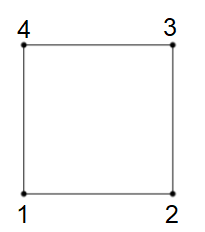
\includegraphics[width=0.25\textwidth, height=0.25\textwidth]{base_element.png}}
	\caption{Линейный прямоугольный конечный элемент}
	\label{base_element}
\end{figure}
\begin{figure}[!htbp]
	\center{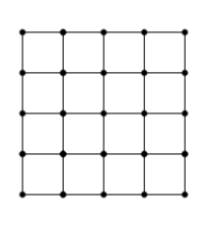
\includegraphics[width=0.25\textwidth, height=0.25\textwidth]{base_element_proection.png}}
	\caption{Проекция расчётной области}
	\label{base_element_proection}
\end{figure}

Пусть $l$ --- горизонтальная длинная области, а $h$ --- вертикальная. Тогда функции формы будут иметь следующий вид:
\begin{equation}
	\begin{cases}
		N_1 = 1 - \frac{x}{l} - \frac{z}{h} + \frac{x  z}{l  h}, \\
		N_2 = \frac{x}{l} - \frac{x  z}{l  h}, \\
		N_3 = \frac{x  z}{l h}, \\
		N_4 = \frac{z}{h} - \frac{x  z}{l  h}. \\
	\end{cases}
\label{form-func}
\end{equation}

\noindent
Аппроксимирующую функцию зададим в виде:
\begin{equation*}
	\phi = c_0 N_1 + c_1 N_2 + c_2 N_3 + c_3 N_4.
\end{equation*}
\noindent
Далее будем искать локальную матрицу из выражения:
\begin{equation}
	\label{init_eq}
	\int_{S_i} {[N]^T \left(\frac{\partial}{\partial x} \left(h^3 \frac{\partial p}{\partial x} \right) + \frac{\partial}{\partial z} \left(h^3 \frac{\partial p}{\partial z} \right) - 6 \mu U \frac{\partial h}{\partial x}\right) dx dz} = 0.
\end{equation}
$S_i$ --- область, содержащая элемент. 
Подставим аппрокисимирующую функцию $\phi$ вместо $p$.
\begin{equation*}
	\int_{S_i} {[N]^T \left(\frac{\partial}{\partial x} \left(h^3 \frac{\partial \phi}{\partial x} \right) + \frac{\partial}{\partial z} \left(h^3 \frac{\partial \phi}{\partial z} \right) - 6 \mu U \frac{\partial h}{\partial x}\right) dx dz} = 0.
\end{equation*}
Понизим порядок производной с помощью функции дифференцирования произведения:
\begin{equation*}
	 \frac{\partial}{\partial x} \left( [N]^T h^3 \frac{\partial \phi}{\partial x} \right)  = [N]^T \frac{\partial}{\partial x} \left(h^3 \frac{\partial \phi}{\partial x} \right) + \frac{\partial[N]^T}{\partial x} \left(h^3 \frac{\partial \phi}{\partial x} \right),
\end{equation*}
\begin{equation*}
	 \frac{\partial}{\partial z} \left( [N]^T h^3 \frac{\partial \phi}{\partial z} \right)  = [N]^T \frac{\partial}{\partial z} \left(h^3 \frac{\partial \phi}{\partial z} \right) + \frac{\partial[N]^T}{\partial z} \left(h^3 \frac{\partial \phi}{\partial z} \right).
\end{equation*}

Подставим полученные выражения в исходный интеграл~\eqref{init_eq}:
\begin{equation*}
\int_{S_i} {\left(\frac{\partial}{\partial x} \left( [N]^T h^3 \frac{\partial \phi}{\partial x} \right) - \frac{\partial[N]^T}{\partial x} \left(h^3 \frac{\partial \phi}{\partial x} \right) \right) dxdz} + 
\end{equation*}
\begin{equation*}
 + \int_{S_i} {\left(\frac{\partial}{\partial z} \left( [N]^T h^3 \frac{\partial \phi}{\partial z} \right) - \frac{\partial[N]^T}{\partial z} \left(h^3 \frac{\partial \phi}{\partial z} \right) - [N]^T 6 \mu U \frac{\partial h}{\partial x}\right) dxdz} = 0.
\end{equation*}

С помощью формулы Грина можно заменить третье и первое слагаемое под знаком интеграла
\begin{equation*}
	\int_{S_i} {\left(\frac{\partial}{\partial x} \left( [N]^T h^3 \frac{\partial \phi}{\partial x} \right) + \frac{\partial}{\partial z} \left( [N]^T h^3 \frac{\partial \phi}{\partial z} \right)  \right)   dxdz} =
\end{equation*}
\begin{equation*}
	= \oint_{\partial S_i} { \left( [N]^T h^3 \frac{\partial \phi}{\partial x} l_x +   [N]^T h^3 \frac{\partial \phi}{\partial z} l_z \right)  d \left( \partial S_i \right)}.
\end{equation*}

Выражение~\eqref{init_eq} примет вид:
\begin{equation*}
	\oint_{\partial S_i} { \left( [N]^T h^3 \frac{\partial \phi}{\partial x} l_x +   [N]^T h^3 \frac{\partial \phi}{\partial z} l_z \right)  d \left( \partial S_i \right)} -
\end{equation*}
\begin{equation*}
	- \int_{S_i} {\left( \frac{\partial[N]^T}{\partial x} \left(h^3 \frac{\partial \phi}{\partial x} \right) +  \frac{\partial[N]^T}{\partial z} \left(h^3 \frac{\partial \phi}{\partial z} \right) - [N]^T 6 \mu U \frac{\partial h}{\partial x}\right) dxdz} = 0.
\end{equation*}

Поскольку в условии задачи заданы граничные условия, то можно не учитывать интеграл по границе. Узлы на которые влияет этот интеграл будут совпадать с узлами, которые зафиксированы граничными условиями.

Итоговое уравнение~\eqref{init_eq} будет иметь вид:
\begin{equation*}
	\int_{S_i} {\left( \frac{\partial[N]^T}{\partial x} \left(h^3 \frac{\partial \phi}{\partial x} \right) +  \frac{\partial[N]^T}{\partial z} \left(h^3 \frac{\partial \phi}{\partial z} \right) - [N]^T 6 \mu U \frac{\partial h}{\partial x}\right) dxdz} = 0.
\end{equation*}

После вычислений этих интегралов можно получить матричное уравнение в локальных координатах относительно $\phi$ следующего вида:
\begin{equation}
W_i \phi = F_i,
\label{ref_local}
\end{equation}
где $F_i$ - правая часть, полученная из интеграла, не содержащего $\phi$:
\begin{equation*}
	F_i = \int_{S_i} [N]^T\left(6 \mu U \frac{\partial h}{\partial x}\right) dx dz.
\end{equation*}

Для вычисления глобальной матрицы требуется для каждого элемента подставить в вырождение~(\ref{ref_local}) для локальных координат узловые границы области и вычислить их значения. 
Далее нужно объединить все матрицы полученные в одну глобальную. Этот процесс будет описан более подробно позже.
После объединения локальных матриц в глобальную получаем матричное уравнение 
\begin{equation*}
	W \phi = F,
\end{equation*}

Далее заменяем значения в матрице $F$ и матрице $W$ так, чтобы значения в граничных узлах совпадали с граничными условиями.
После этого решением уравнения будут являться искомые значения давления $p$ в узловых точках.

\subsection{Построение метода конечных элементов}
В работе уже был описан принцип решения решения уравнения Рейнольдса с помощью слабой формы Галеркина, однако его программная реализация требует дополнительных пояснений.

Для вычисления нового конечного элемента получаются интегралы согласно слабой формы Галеркина в локальной системе координат. Вычисление интегралов необходимо на каждом шаге, поскольку требуется преобразовать функцию зазора $h$ из глобальных координат в локальные, задавая смещение по оси $x$.

Затем происходит вычисление значений узлов конечных элементов, учет граничных условий и их объединение. Так много действий объединено в один этап, поскольку в ином случае для выполнения всех перечисленных действий требовались бы дополнительные вычислительные затраты и использование дополнительной памяти для хранения информации о структуре полученных узлов. Для иллюстрации будем рассматривать решение для сетки с 2 элементами по вертикали и 2 по горизонтали.

Итак, вычисления происходят следующим образом: вначале рассчитывается самый нижний левый конечный элемент. В качестве результата вычисления одного элемента получаем систему из 4 однородных уравнений. Записываем полученную систему в массив решений и сохраняем данные об индексах двух крайних правых узлах \{2,~3\} и двух верхних \{3,~4\}. Важно, что крайние правый элемент мы будем хранить только для самого последнего вычисленного элемента, а значение индексов верхних узлов для всего ряда конечных элементов. По какой причине это происходит именно так стане яснее на следующих этапах вычисления. Поскольку мы имеем граничные условия по условию задачи, то для граничных узлов имеет смысл сразу их учесть. Граничными узлами для рассматриваемого элемента будут являться узлы \{1,~2,~4\}. Заменим уравнения в системе, соответствующие этим узлам, так, чтобы они удовлетворяли граничным условиям. В программе это реализовано в виде уравнения $nodeValue - boundaryValue = 0$, где $nodeValue$ --- неизвестное значение в узле, а $boundaryValue$ --- граничное значение. 
\begin{figure}[!htbp]
	\center{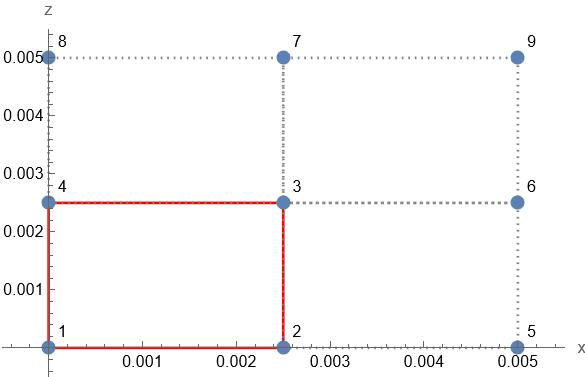
\includegraphics[width=0.7\textwidth, height=0.5\textwidth]{left-bottom-el.jpg}}
	\caption{Нижний левый конечный элемент на сетке 2 на 2 элементов}
	\label{left-bottom-el}
\end{figure}

Далее в цикле вычисляем все оставшиеся конечные элементы в этом ряду, на выбранной сетке он всего один. Поскольку новых узлов в сетке будет всего два, то необходимо будет использовать те же переменные для обозначения уже используемых узлов сетки. Как раз для этого и было сохранено значение индексов крайне правых элементов. Для осуществления слияния двух узлов разных конченых элементов уравнения для этих узлов складываются. В случае, если общие узлы оказываются граничными, то в сложение уравнений смысла не имеет - они и так отвечают граничным условиям. Добавляем в массив индексов верхних элементов новую пару узлов и сохраняем новые крайние правые узлы аналогично прошлому этапу. Аналогично с прошлым этапом учитываем граничные условия
\begin{figure}[!htbp]
	\center{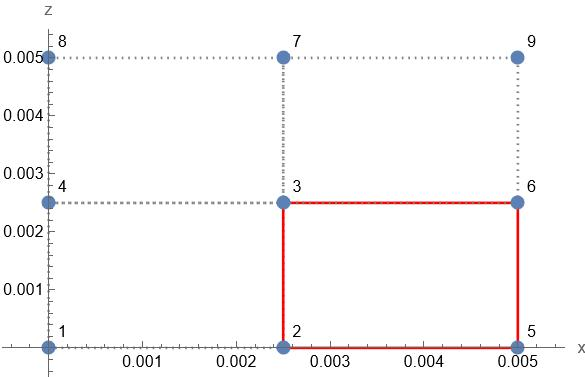
\includegraphics[width=0.7\textwidth, height=0.5\textwidth]{right-bottom-el.jpg}}
	\caption{Нижний правый конечный элемент на сетке 2 на 2 элементов}
	\label{right-bottom-el}
\end{figure}
\newpage
После этого переходим к вычислению конечных элементов выше по оси $z$.  Для этого будет использоваться цикл по вертикальной оси $z$. В рассматриваемом случае в этом цикле будет всего один ряд элементов, лежащих между 0.003 и 0.005 по оси $z$.
Рассмотрим вычисление элемента с узлами \{4,~3,~7,~8\}. Для него большая часть действий аналогично, не будем их повторять. Главной отличительной чертой алгоритма относительно прошлых конечных элементов будет использования массива индексов верхних узлов, который был заполнен на ранних этапах. Он нужен добавления в систему решения общих нижних узлов элементов - \{4,~3\}. Добавление происходит путем складывания имеющегося уравнения в системе с новым уравнением для вычисляемого узла. После все вычислений мы как и ранее сохраняем значение крайне правых узлов и обновляем индекс для крайне верхних узлов в массиве. Стоит заметить, что массив индексов крайне верхних узлов имеет размерность равную числу горизонтальных элементов сетки, то есть размерность 2 для рассматриваемого случае. В нем хранятся только актуальные для вычисления индексы.
\begin{figure}[!htbp]
	\center{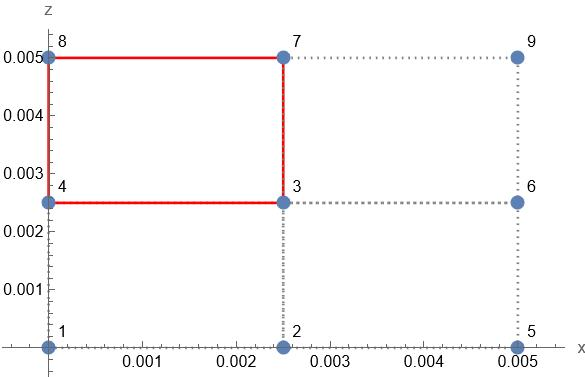
\includegraphics[width=0.7\textwidth, height=0.5\textwidth]{left-top-el.jpg}}
	\caption{Верхний левый конечный элемент на сетке 2 на 2 элементов}
	\label{left-top-el}
\end{figure}
\newpage
Для получения последующих уравнений для узлов конченых элементов используется цикл по оси $x$. Каких-то новых приемов для его вычисления не используется, расчет ведется аналогично с прошлыми элементами. В рассматриваемом случае такой элемент всего один.
\begin{figure}[!htbp]
	\center{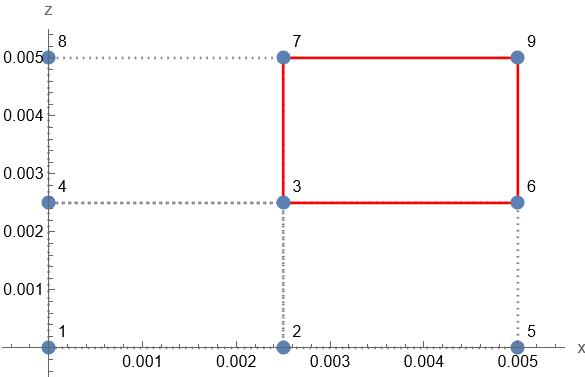
\includegraphics[width=0.7\textwidth, height=0.5\textwidth]{right-top-el.jpg}}
	\caption{Верхний правый конечный элемент на сетке 2 на 2 элементов}
	\label{right-top-el}
\end{figure}

Итого получаем систему линейных алгебраических уравнений, которая позволит получить нам давления в каждом из узлов сетки. Решаем систему с помощью встроенной в Wolfram Mathematica функции Solve и получаем решение задачи -- набор значений давлений в заданных узлах сетки.

\subsection{Верификация программы на основе обратной подстановки}
В качестве первого способа проверки вначале зададим функцию решения, вычислим для нее правую часть и затем подставим полученную правую часть в нашу программу. Так мы сможем сравнить полученное решение со значениями функции заданной нами самими.

В качестве первой проверочной функции рассмотрим
\begin{equation}
	f(x, z) = -2 \frac{\pi }{0.005} \sin{\left(\frac{\pi z}{0.005}\right)} x \left(x - 0.005\right)
	\label{check_func_1}
\end{equation}
\begin{figure}[!htbp]
	\center{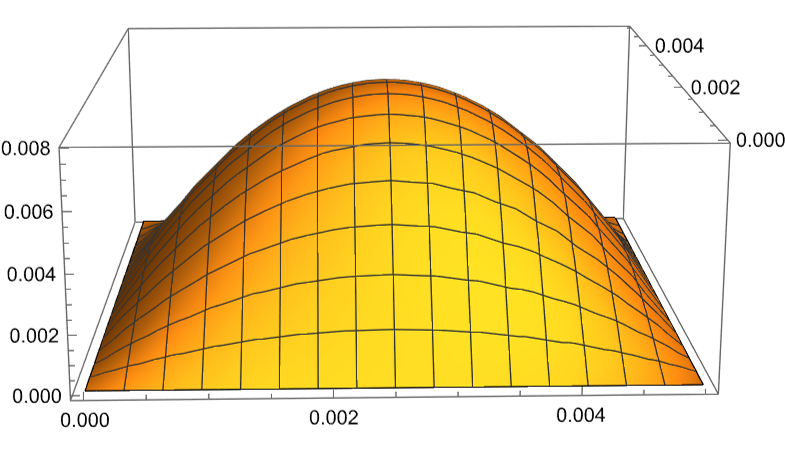
\includegraphics[width=0.7\textwidth, height=0.5\textwidth]{check_func_1.png}}
	\caption{Первая проверочная функция~\eqref{check_func_1}}
	\label{check_func_1_pic}
\end{figure}
Далее вычислим правую часть подставив~\eqref{check_func_1} в уравнение
\begin{equation*}
	F = \frac{\partial^2 f}{x^2} + \frac{\partial^2 f}{\partial z}
\end{equation*}
Полученную правую часть подставим в программу и будем искать искомую функцию $f$.

\begin{table}[!htbp]
	\begin{tabular}{|l|l|l|}
		\hline
		\multicolumn{1}{|c|}{Размерность сетки} & \multicolumn{1}{c|}{Разность, Па} & Погрешность, \% \\ \hline
		5 на 5                                  & 0.969                              & 21.31            \\ \hline
		10 на 10                                & 0.260                              & 5.7            \\ \hline
		20 на 20                                & 0.065                              & 1.4            \\ \hline
	\end{tabular}
\end{table}

\begin{figure}[!htbp]
	\center{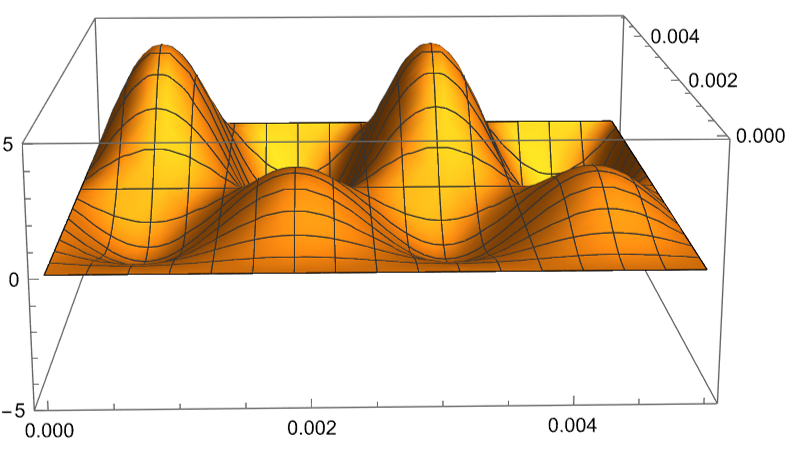
\includegraphics[width=0.7\textwidth, height=0.5\textwidth]{check_func_2.png}}
	\caption{Результат вычислений для проверочной функции~\eqref{check_func_1} на сетке 20 на 20}
	\label{res_check_func_1}
\end{figure}


В качестве второй проверочной функции рассмотрим
\begin{equation}
	f(x, z) = -2 \frac{\pi z}{0.005} \sin{\frac{2 \pi z}{0.005}} \sin{\frac{4 \pi x}{0.005}}
	\label{check_func_2}
\end{equation}
\begin{figure}[!htbp]
	\center{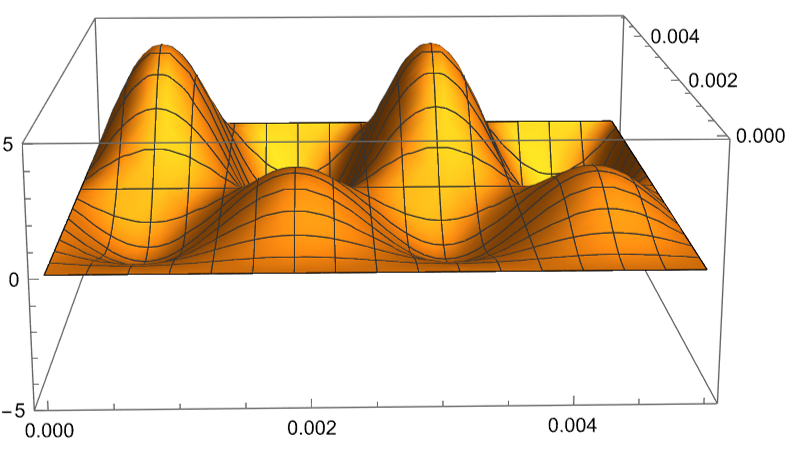
\includegraphics[width=0.7\textwidth, height=0.5\textwidth]{check_func_2.png}}
	\caption{Вторая проверочная функция~\eqref{check_func_2}}
	\label{check_func_2_pic}
\end{figure}
Как видно значение функции на границах нулевое.

Аналогичным образом получим правую часть и подставим ее в программу.

\begin{table}[!htbp]
	\begin{tabular}{|l|l|l|}
		\hline
		\multicolumn{1}{|c|}{Размерность сетки} & \multicolumn{1}{c|}{Разность, Па} & Погрешность, \% \\ \hline
		5 на 5                                  & 0.969                              & 21.31            \\ \hline
		10 на 10                                & 0.260                              & 5.7            \\ \hline
		20 на 20                                & 0.065                              & 1.4            \\ \hline
	\end{tabular}
\end{table}

Погрешность была вычислена по формуле $\underset{i}{\max} | \frac{{x_t}_i - {x_{node}}_i}{{x_t}_i} |$, где ${x_t}_i$ -- значение в узле $i$, полученное из искомой функции, а ${x_{node}}_i$ -- значение в узле $i$, полученное в программе. Максимум вычисляется по всем узловым элементам.

Итого можно делать вывод, что на приведенных примерах программа считает верно, погрешность сокращается с увеличением числа элементов на сетке. Из двух проверок можно видеть, что для первой более простой по форме функции достаточно 10 элементов для получения небольшой погрешности, тогда как для более сложной второй функции нужно не мена сетка 20 элементов.

\begin{figure}[!htbp]
	\center{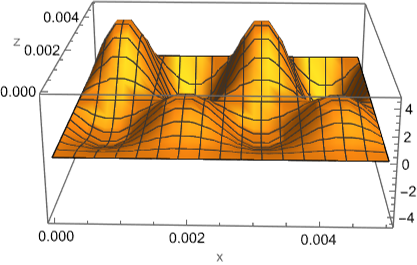
\includegraphics[width=0.7\textwidth, height=0.5\textwidth]{res_check_func_2.png}}
	\caption{Результат вычислений для проверочной функции~\eqref{check_func_2} на сетке 20 на 20}
	\label{res_check_func_2}
\end{figure}



\subsection{Верификация программы путем сравнения с Wolfram Mathematica}

Проверим полученный результат с помощью функции NDSolve в Wolfram Mathematica.

\begin{figure}[!htbp]
	\center{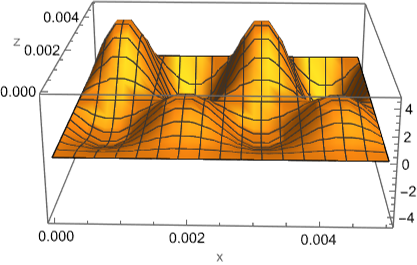
\includegraphics[width=0.\textwidth, height=0.5\textwidth]{res_check_func_2.png}}
	\caption{График решения уравнения Рейнольдса для h = 0.0001 м полученный с помощью Wolfram Mathematica}
	\label{exactSolutionConst}
\end{figure}

Сравним решения полученные с помощью собственной реализацией с решением Wolfram Mathematica.

\begin{table}[!htbp]
	\begin{tabular}{|l|l|l|}
		\hline
		\multicolumn{1}{|c|}{Размерность сетки} & \multicolumn{1}{c|}{Разность, Па} & Погрешность, \% \\ \hline
		5 на 5                                  & 4612                              & 4.51            \\ \hline
		10 на 10                                & 1538                              & 1.38            \\ \hline
		20 на 20                                & 1290                              & 1.02            \\ \hline
	\end{tabular}
\end{table}

Можно заметить, что полученное решение отличается не более чем на 4.51 \%, с увеличением числа элементов в сетке погрешность падает. Это свидетельствует о верности полученного решения. 

Верификация работы программы была произведена двумя способами, таким образом можно судить о верности работы программы.

\subsection{Результаты моделирования}

Для демонстрации результатов рассмотрим различные функции зазора $h(x)$.  Расчеты будем проводить на сетке 10 на 10 со стандартными параметрами указанными в постановке задачи~\eqref{reinolts-task}.

В начале вычислим давление для постоянного зазора
\begin{figure}[!htbp]
	\center{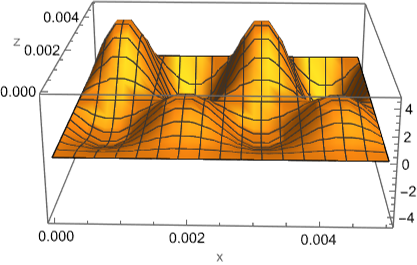
\includegraphics[width=0.\textwidth, height=0.5\textwidth]{res_check_func_2.png}}
	\caption{График решения уравнения Рейнольдса для h = 0.001 м}
	\label{sol_const_h}
\end{figure}

Затем получим график для увеличивающегося зазора
\begin{figure}[!htbp]
	\center{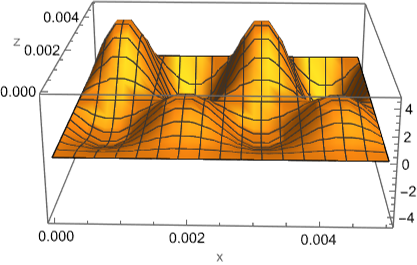
\includegraphics[width=0.\textwidth, height=0.5\textwidth]{res_check_func_2.png}}
	\caption{График решения уравнения Рейнольдса для h = 0.15 x + 0.001 м}
	\label{sol_pos_h}
\end{figure}

Так выглядит давление на пластину для уменьшающегося зазора
\begin{figure}[!htbp]
	\center{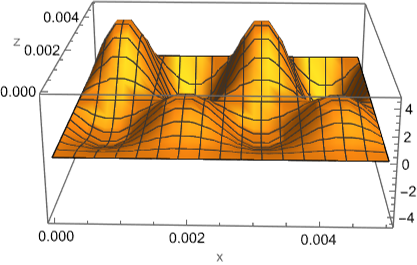
\includegraphics[width=0.\textwidth, height=0.5\textwidth]{res_check_func_2.png}}
	\caption{График решения уравнения Рейнольдса для h = 0.15 x + 0.001 м}
	\label{sol_neg_h}
\end{figure}

Чтобы более наглядно увидеть отличия которые вызывает знак перед коэффициентом у $x$ построим графики с одинаковыми граничными условиями на всех гранях равными $100000$ Па.

При положительном коэффициенте видимо провал
\begin{figure}[!htbp]
	\center{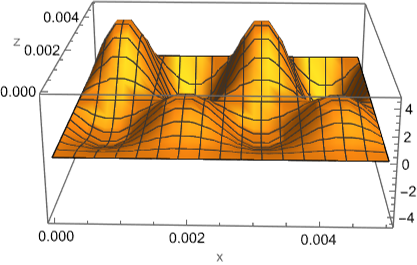
\includegraphics[width=0.\textwidth, height=0.5\textwidth]{res_check_func_2.png}}
	\caption{График решения уравнения Рейнольдса для h = 0.15 x + 0.001 м}
	\label{sol_pos_h}
\end{figure}

При отрицательном коэффициенте наблюдаем пик
\begin{figure}[!htbp]
	\center{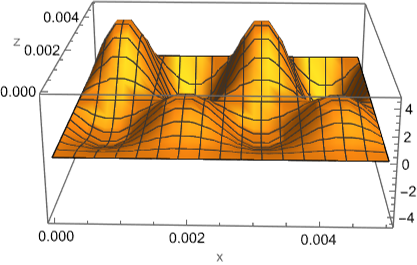
\includegraphics[width=0.\textwidth, height=0.5\textwidth]{res_check_func_2.png}}
	\caption{График решения уравнения Рейнольдса для h = 0.15 x + 0.001 м}
	\label{sol_pos_h}
\end{figure}

\newpage
\section{Аэроупругая модель}
Для построения аэроупругой модели не достаточно получить решение уравнения Рейнольдса. Для ее получения необходимо дополнить имеющуюся модель пружиной, ограничивающей движение пластины сверху. Закрепим пружину по центру пластины в точке $\{0.0025, 0.0025\}$. 

\begin{figure}[!htbp]
	\center{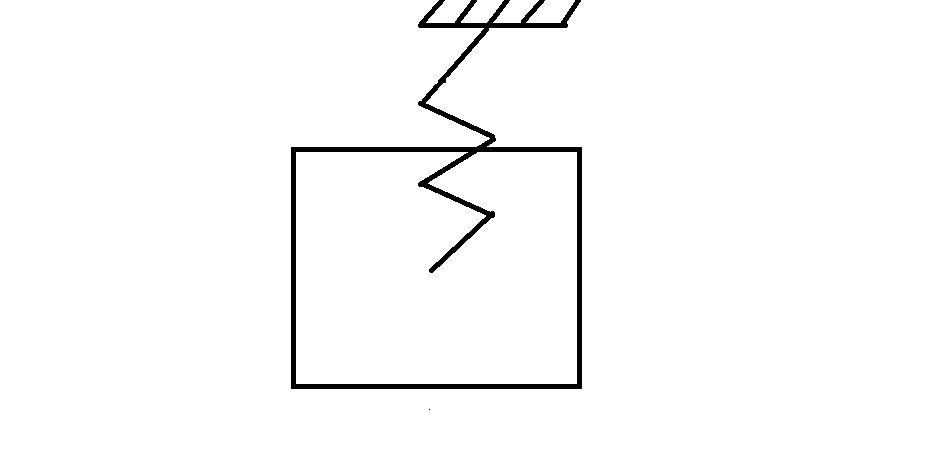
\includegraphics[width=0.\textwidth, height=0.5\textwidth]{pruzina.png}}
	\caption{График решения уравнения Рейнольдса для h = 0.15 x + 0.001 м}
	\label{pruzina}
\end{figure}


Необходимо связать изменения положения пластины и сжатия и растяжение пружины.


\newpage
\section-{Заключение}
В работе представлен вывод уравнения Рейнольдса для установившегося течения в газовом смазочном слое и методика решения уравнения Рейнольдса с помощью метода конечных элементов. В ходе работы получены следующие результаты:
	\begin{enumerate}	
		\item Создана программная реализация метода конечных элементов для решение уравнения Рейнольдса
		\item Полученные значения решения уравнения Рейнольдса были сравнены с результатами решения, полученного с помощью функции NDSolve в Wolfram Mathematica
		\item В результате сравнения для сетки 5 на 5 погрешность равна 4.51 \%, а для сетки 20 на 20 -- 1.02 \%.
	\end{enumerate}

\newpage
\begin{thebibliography}{2}
\bibitem{petrov_smazka} Петров Н. Гидродинамическая теория смазки, М.: из-во академии наук СССР, 1948. --- 558~с.
\bibitem{slezkin_smazka} Слезкин Н. Динамика вязкой несжимаемой жидкости, М.: из-во техно-теоретической литературы, 1955. --- 521~с.
\bibitem{seligard} Селегринд Л. Примененение метода конечных элементов, М.: из-во МИР, 1979. --- 195~с.
\bibitem{seshu} Seshu P. Textbook of
Finite Element
Analysis, New Dehli: PHI Learning Private Limited, 2012. --- 340~с.
\bibitem{itmo} Григорьев А. Колебания
и виброактивность элементов машин: Учеб. пособие. СПб.: Университет ИТМО, 2016. --- 136~с.

\end{thebibliography}

\newpage

\section-{Приложение А}

\end{document} 